\chapter{Recherche und Installation des Groupware-Systems}

In diesem Kapitel wird der Prozess der Recherche und Installation des Groupware-Systems beschrieben.
Dabei wird zuerst auf die Kriterien für das Groupware-System eingegangen, die im Laufe der Recherche berücksichtigt wurden.
Anschließend werden die betrachteten Groupware-Systeme vorgestellt und die Entscheidung für ein System begründet.
Zuletzt wird die Installation des Groupware-Systems auf einer Cloud-Instanz beschrieben.

\section{Kriterien für das Groupware-System}
\begin{itemize}
    \item \textbf{Open Source:} 
    Das erste und wichtigste Kriterium ist, dass das Groupware-System Open Source ist.
    Daher werden im Laufe der Recherche nur Open Source Groupware-Systeme betrachtet.
    \item \textbf{Eigenverwaltbarkeit:}
    Die Hochschule Esslingen hat ein eigenes Rechenzentrum und eine IT-Fakultät.
    Daher sollte die Software von der Hochschule Esslingen selbst installiert und administriert werden können.
    \item \textbf{Deutsche Firma:}
    Als deutsche Hochschule möchte die Hochschule Esslingen auch deutsche Firmen unterstützen.
    Deshalb ist es eine Vorgabe, dass das Groupware-System von einer deutschen Firma entwickelt wird.
    Dies ist zwar ein wichtiges Kriterium, muss aber nicht zwingend zum Ausschluss führen.
    \item \textbf{Automatisierbarkeit:}
    Teile der Konfiguration des Groupware-Systems, wie beispielsweise das Hinzufügen und die Konfiguration von Nutzern, sollen automatisierbar sein.
    Das soll das Hinzufügen und Entfernen der vielen Nutzer, die an der Hochschule Esslingen beschäftigt sind, erleichtern.
\end{itemize}

\newpage

\section{Betrachtete Groupware-Systeme}

Zu Beginn der Studienarbeit wurden anhand der gegebenen Kriterien mehrere Kandidaten für das Groupware-System recherchiert, um einen Überblick über die verfügbaren Möglichkeiten zu erhalten.
Im folgenden Abschnitt werden die 4 vielversprechendsten Groupware-Systeme der ersten Recherche, Kolab, Horde, Sogo und EGroupware, mit ihren Funktionalitäten und anderen relevanten Informationen vorgestellt.
Dabei wird auch auf die Verbreitung der Systeme an anderen Organisationen, vor allem aber Hochschulen und Universitäten, eingegangen.
Das soll eine erste Einschätzung über die Eignung der Systeme zur eigenen Verwaltung durch die Hochschule geben.


\subsection{Kolab}

Das Groupware-System Kolab wird von der Schweizer Firma Aphelia IT AG entwickelt und ist als Open-Source Produkt gratis verfügbar und bietet die folgenden Features:
\begin{itemize}
    \item E-Mail
    \item Kalender
    \item Kontakte
    \item Online-File-Server
    \item Aufgabenmanagement
    \item Notizen
    \item Sprach- und Videoanrufe
\end{itemize}
\autocite[Quelle:][]{kolab}

Kolab wird von der Firma Nestlé und der Universität Tübingen verwendet und ist daher auch für größere Organisationen geeignet.

\subsection{Horde}

Horde wird von einem gleichnamigen amerikanischen Unternehmen entwickelt und ist wie die anderen Systeme Open-Source und gratis verfügbar. Es bietet dabei die folgenden Funktionalitäten:
\begin{itemize}
    \item E-Mail
    \item Kalender
    \item Kontakte
    \item Online-File-Server
    \item Terminmanagement
    \item Projektmanagement
    \item Dokumentenmanagement
    
\end{itemize}
\autocite[Quelle:][]{horde}

Relevant für die Auswahl könnte auch sein, dass Horde schon von einigen anderen Universitäten und Hochschulen, wie beispielsweise der Universität Tübingen und Universität Paderborn, verwendet wird.

\subsection{Sogo}

Sogo ist ein Open-Source Groupware-System, welches von der französischen Firma Alinto entwickelt wird.
Das System ist frei verfügbar und bietet die folgenden Features:

\begin{itemize}
    \item E-Mail
    \item Kalender
    \item Kontakte
    \item Erinnerungen
    \item 2-Faktor-Authentifizierung
    \item Raum Reservationen
\end{itemize}
\autocite[Quelle:][]{sogo}

Ähnlich wie Horde wird auch Sogo von einigen Universitäten und Hochschulen verwendet, wie beispielsweise der Universität Koblenz und der Universität Ulm.

\subsection{EGroupware}

EGroupware ist ein Open-Source Groupware-System, welches von einer deutschen Firma entwickelt wird.

Als Funktionalitäten bietet EGroupware:

\begin{itemize}
    \item E-Mail
    \item Kalender
    \item Kontakte
    \item Online-File-Server
    \item Terminmanagement
    \item Projektmanagement
    \item Dokumentenmanagement
\end{itemize}

Auch EGroupware wird von einigen Hochschulen genutzt, jedoch von deutlich weniger als die anderen Systeme.


\section{Entscheidung für ein Groupware-System}

Bei der Recherche der verschiedenen Groupware-Systeme wurde klar, dass alle der untersuchten Systeme die grundlegenden gewünschten Funktionalitäten bieten und daher grundsätzlich alle für die Hochschule Esslingen geeignet sind.
Durch diesen Umstand konnte die Entscheidung nicht rein aufgrund der Funktionalitäten der Systeme getroffen werden, da sich keines der Systeme in diesem Punkt stark von den anderen abhebt.
Somit fiel final die Entscheidung auf EGroupware, da es von einer deutschen Firma entwickelt wird und umfangreiche Funktionen bietet, die für die Hochschule Esslingen relevant sein könnten.




\section{Installation auf der Cloud}

Für die Installation der EGroupware Software stellt die EGroupware GmbH eine Installationsanleitung zu Verfügung.
Darin wird auf einer Linux Instanz zunächst ein Docker Repository hinzugefügt und anschließend die EGroupware Software in Form von 5 Docker Containern installiert und gestartet.
Alle dafür benötigten Konsolenbefehle waren in der Installationsanleitung angegeben. \autocite{egroupware-installation}

Für das Hosting der EGroupware Software wurde sowohl WSL2 (Windows-Subsystem für Linux) als auch eine bwCloud Instanz getestet.
Die reine Installation der Software verlief auf beiden Systemen auf einer Ubuntu22.04 Instanz ohne Probleme.
Im Laufe der Konfiguration wurde jedoch klar, dass die Netzwerkkonfiguration bei bwCloud einfacher zu handhaben ist als bei WSL2.
Daher wurde die finale Installation und Konfiguration auf einer bwCloud Instanz durchgeführt.
Damit das Frontend der Software über das Internet erreichbar ist, muss Port 80 für HTTP Kommunikation freigegeben werden.
Das wurde wie in Abbildung \ref{fig:bwcloud_security_group} gezeigt in einer benutzerdefinierten Sicherheitsgruppe der bwCloud Instanz realisiert.
\begin{figure}[H]
    \centering
    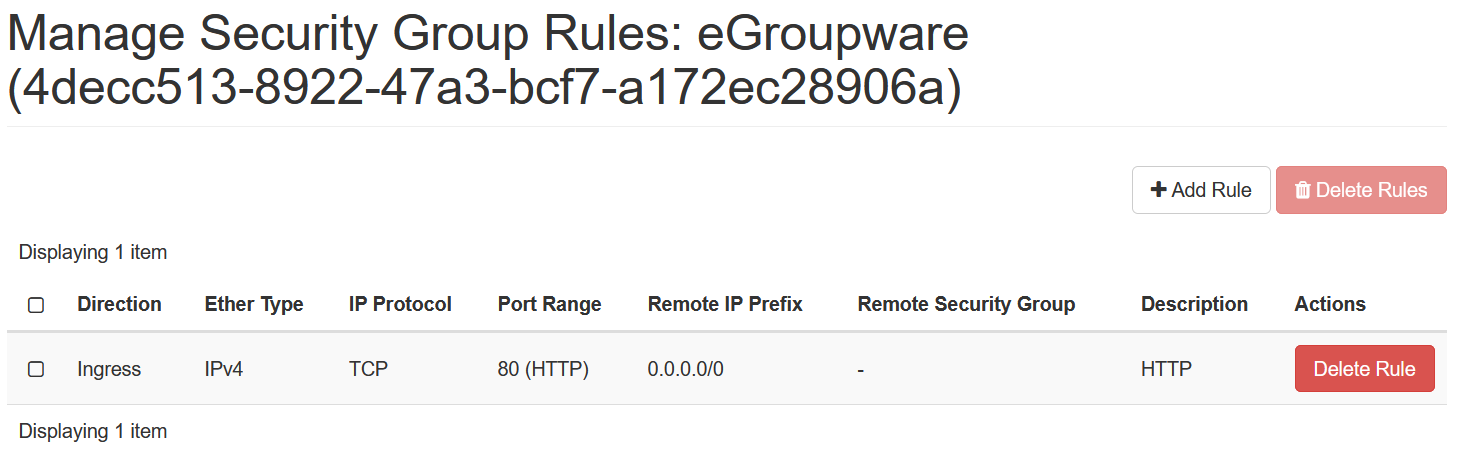
\includegraphics[width=0.75\textwidth]{images/bwCloud_SecurityGroup.png}
    \caption{Konfiguration der Sicherheitsgruppe für die bwCloud Instanz von EGroupware}
    \label{fig:bwcloud_security_group}
\end{figure}

Für die grundlegende Konfiguration der Software, wie beispielsweise das Konfigurieren von LDAP oder SAML 2.0, bietet die EGroupware Software ein Setup-Tool, welches über folgende URL erreichbar ist:

\fbox{\texttt{http://host-or-ip/egroupware/setup/}}

Für den ersten Zugriff auf die tatsächliche Software für beispielsweise das Erstellen von Nutzer Accounts wird bei der Installation automatisch ein Administrator Account angelegt, dessen Zugangsdaten im Log der Installation zu finden sind.
Das Frontend der Groupware ist dann über die folgende URL erreichbar:

\fbox{\texttt{http://host-or-ip/egroupware/login.php/}}
